\chapter{Introduction}
\label{chap:introduction}

In the most general sense, the problem of segmentation is the challenge of how to partition an object into pieces in such a way as to ensure that those pieces have some meaning in a given domain. The related (and to some extent overlapping) problem of feature identification is how to then ascribe meaning to some or all of those pieces. Whilst a huge variety of techniques have been developed for these problems, there are many domains in which it is difficult to specify, at least in a sufficiently precise manner, what constitutes a meaningful piece and what does not. For that reason, both problems remain major research challenges.

Nevertheless, an ability to solve these problems, even in an imperfect way, is often a crucial precursor to applying other algorithms in various domains, making them worthy targets for research efforts. For example, in the medical imaging domain, it is helpful to be able to translate a volume of data produced by a scanner into a 3D mesh, allowing doctors to visualize the state of a patient's organs in a more direct manner. Whilst there are existing algorithms to convert \emph{labelled} volume data to a 3D mesh (e.g.~\cite{wu03}), these rely on \emph{a priori} knowledge of the location of the organs. That is, they rely on the organs having being labelled in the volume in advance. Producing such a labelling is a segmentation and feature identification problem.

This thesis is about tackling the segmentation and feature identification problems for a particular type of medical image, namely computerised tomography (CT) scans of a patient's abdomen. The first practical CT scanner was developed in 1971 by Sir Godfrey Hounsfield, working at the EMI Central Research Laboratories in Hayes, UK.\footnote{Credit for the CT technique is also due to Allan McLeod Cormack of Tufts University in Massachusetts in the United States, who independently developed the theory underpinning CT in the late 1950s and early 1960s. Both men shared the 1979 Nobel Prize in Physiology or Medicine.} CT scanners work using X-rays and produce images whose pixels are scalar values on a scale of radiodensity known (after Sir Godfrey) as the Hounsfield scale. They are used extensively in modern medical practice \cite{garvey02}, both for diagnosing illness and for evaluating a patient's response to therapy.

%---
\stufigex{height=8cm}{introduction/introduction-labelledabdominalscan.png}{An abdominal CT scan of a patient with a large renal tumour on their left kidney. Some of the key features in the scan are labelled.}{fig:introduction-labelledabdominalscan}{t}
%---

My underlying interest is in renal (kidney) cancers, in the diagnosis of which CT scanners are generally used to produce images of the abdomen (see Figure~\ref{fig:introduction-labelledabdominalscan}). Whilst less prevalent than some other types of cancer -- notably breast, lung, colorectal and prostate -- renal cancers nevertheless kill thousands of people a year in the UK.\footnote{According to Cancer Research UK \cite{cruk-kidneycancermortality}, 3752 people died from a kidney cancer in the UK in 2007, the most recent year for which published statistics are currently available.} An ability to visualize the state of a renal cancer patient's abdominal organs in 3D can provide doctors with an extra tool when making important decisions about how best to treat the patient. In a similar vein, being able to calculate the volume of a renal tumour can help doctors track changes over time that may be relevant when evaluating a patient's response to therapy. For these, and other, applications, finding a way to segment and identify features in abdominal CT scans is a key prerequisite.

%---
\stufigex{height=6cm}{introduction/introduction-campadelli.png}{An example output of the fully-automatic technique to identify abdominal organs described in \cite{campadelli09} (extracted from Figure 7 of that paper), showing the excellent results they obtained when automatically identifying the bones, heart and kidneys.}{fig:introduction-campadelli}{t}
%---

Given the relevance of the abdominal CT segmentation and feature identification problems, it is unsurprising that significant research effort has been devoted to them in recent years. Approaches range from manual, where the user is required to draw round the relevant features in every slice, to semi-automatic, where the user has to do some of the segmentation work but can then leave the rest to the computer (e.g.~\cite{loncaric00}), to fully-automatic, where abdominal features are extracted with no relevant user interaction. Two particularly noteworthy fully-automatic methods are \cite{campadelli09} and \cite{shimizu07}. In \cite{campadelli09}, Campadelli et al.\ described a grey-level based framework that allowed them to automatically extract the bones, heart, kidneys, liver (including its blood vessels) and spleen from CT scans (e.g.~see Figure~\ref{fig:introduction-campadelli}), an approach they tested on images from $100$ patients. Full validation was done for the liver and spleen, by comparing the output to three expert ground truth segmentations, with excellent results being achieved for those organs. In \cite{shimizu07}, Shimizu et al.\ proposed an atlas-guided approach that attempted to automatically extract twelve abdominal features (aorta, gallbladder, heart, inferior vena cava, left kidney, liver, oesophagus, pancreas, portal vein, right kidney, spleen and stomach). Whilst they only tested their approach on images from $10$ patients, they achieved promising results for most of the major organs (see Figure~\ref{fig:introduction-shimizu}). One slight downside is the significant amount of computing power used by their approach (a message passing interface (MPI) implementation running on $16$ 2.8GHz CPUs, each with 4GB of memory), although it seems plausible that this could be reduced.

%---
\stufigex{height=6cm}{introduction/introduction-shimizu.png}{An example output of the fully-automatic technique to identify abdominal organs described in \cite{shimizu07} (extracted from Figure 8 of that paper). Twelve features have been identified: the aorta (pink), gallbladder (light green), heart (yellow), inferior vena cava (red), left kidney (light orange), liver (maroon), oesophagus (purple), pancreas (green), portal vein (light blue), right kidney (orange), spleen (white) and stomach (blue).}{fig:introduction-shimizu}{t}
%---

Despite the evident successes of some current fully-automatic approaches, however, it remains the case that whilst medics may not necessarily want to be forced to interact substantively with a segmentation and feature identification application in its initial stages, they are generally keen to retain the ability to carefully examine and edit its output. For that reason, my own approach described in this dissertation has focused not primarily on the fully-automatic identification of abdominal features (although I have done some work in that direction, as will be described in Chapter~\ref{chap:featureid}), but on a good way of facilitating user editing of automatically-generated segmentation and feature identification results.

My approach is based around the idea of representing images using a hierarchical data structure known as a partition forest (or an \emph{image partition forest}, in this context). Partition forests, described more fully in Chapters~\ref{chap:background} and \ref{chap:ipfs}, are in essence a set of hierarchical partitions of the same object (e.g.~an image). Together with partition \emph{trees}, to which they are closely related, they have been applied to good effect to represent images in other sub-fields of image analysis, e.g.~TODO. It is noticeable, however, that despite their widespread appearance in the literature as an image representation technique (see e.g.~\S\ref{sec:background-partitionhierarchies}), surprisingly little work has been done on how to allow partition forests to be easily edited by the user; one notable exception is \cite{nacken95}, in which Peter Nacken describes a constrained parent switching operation for a partition forest-type data structure (I describe a less constrained version of the same operation in Chapter~\ref{chap:ipfs}). In more recent work, Klava et al.~\cite{klava09} take an interesting approach that allows partitions to be viewed as if sibling nodes in the partition forest had been split or merged, via a scheme of defining a non-horizontal cut across the partition forest structure; however, the results obtained using their split and merge operations are fundamentally limited by the underlying forest structure, which they do not change. One of the contributions made by this dissertation (in Chapter~\ref{chap:ipfs}) is to fill this gap by defining a hierarchy of undoable operations that can be used to mutate partition forests and showing how they can be integrated into an easy-to-use graphical user interface (GUI). It will be demonstrated that the core operations at the lowest level of this hierarchy are minimally-sufficient for partition forest editing: that is, a finite sequence of them can be used to mutate any partition forest of an object into any other partition forest of the same object.

In addition to algorithms that mutate partition forests, it is also necessary to allow users to manage selections of subtrees within them (due to the forests' hierarchical nature, selecting a node in a forest is equivalent to selecting all of the node's children). Whilst it is evidently simple to support the user's selection of individual nodes within a partition forest (and this has been done), there does not currently appear to be any subtree-based partition forest selection technique in the literature. Such a technique is thus presented in detail in Chapter~\ref{chap:ipfs}, along with techniques for updating partition forest selections based on changes to the underlying forest (for example, a selection must update itself in response to a selected node in the forest being split).

Aside from the aforementioned algorithms, attention needs to be paid to how partition forests should be constructed for CT images. The essence of the approach I have used is to segment the (smoothed) gradient magnitude of the image using the well-known watershed transform \cite{beucher90} to produce an initial partition of the image (which becomes the lowest branch layer of the partition forest), and then to run the waterfall transform \cite{marcotegui05} (effectively a series of further watershed transforms) on the result to produce the remainder of the forest layers. When run on a 3D image, this relatively straightforward approach can be used to produce an image partition forest for the whole image. However, it can also be interesting to segment the 3D image on a slice-by-slice basis (in any of the three axis-aligned slice planes), whilst still producing a single image partition forest for the entire volume. To that end, I have developed a forest construction algorithm that will segment subvolumes of the 3D image separately and then combine the results to produce an overall forest for the entire image. The details are described in Chapter~\ref{chap:segmentation}.

Many elements of the forest construction process are interesting in their own right. For instance, I initially implemented the waterfall transform using the approach described by Marcotegui and Beucher in \cite{marcotegui05}, but my colleague Chris Nicholls devised a simpler, functional-style tree-based algorithm which achieved almost identical results \cite{nicholls09}. In addition to implementing an imperative version of this new algorithm in C++, I subsequently also developed my own slightly more complicated waterfall algorithm that additionally accounts for non-minimal plateaux in the minimum spanning tree on which the algorithm is run in a consistent manner (unlike either of the existing algorithms). All three algorithms are described in detail and compared side-by-side in \S\ref{?}.

With the forest constructed to represent the 3D image, it is possible to devise algorithms to automatically identify features within it. In particular, this dissertation presents novel algorithms to identify the spine, spinal cord, ribs, aorta, liver and kidneys in Chapter~\ref{chap:featureid}. The results of all of these algorithms are validated in Chapter~\ref{chap:validation} against ground truth segmentations that have been manually delineated and confirmed as accurate by a radiologist. Whilst some of the identifiers need further refinement to increase their robustness, the overall approach shows promise.

I have implemented all of the described techniques and algorithms in C++. Specifically, two separate systems were developed to do segmentation, feature identification and 3D visualization. The trial system, \emph{centipede}, ran only on Microsoft Windows, and segmented each slice in a CT (or MRI) series into its own separate image partition forest. The user could mark features manually, or identify features such as the ribs and spine automatically in 2D CT images (see Figure~\ref{fig:introduction-centipede}). This work was published in \cite{gvccimi08} and \cite{gvcispa09}, with the former paper receiving the Professor Yasuhiko Dote award for the Best Workshop Paper at the Fifth International Conference on Soft Computing as Transdisciplinary Science and Technology (CSTST '08). It was also possible to visualize the results as a wireframe 3D mesh (generated using the multiple material marching cubes algorithm described in \cite{wu03}).

%---
\stufigex{width=.95\linewidth}{introduction/introduction-centipede.png}{Automatically identifying the ribs and spine in \emph{centipede} and visualizing the feature labelling as a wireframe 3D mesh -- the visible features are the aorta (red), liver (purple), right kidney (yellow) and spine (white).}{fig:introduction-centipede}{t}
%---

%---
\begin{stusubfig}{p}
	\subfigure[\emph{millipede} running on Microsoft Windows]
	{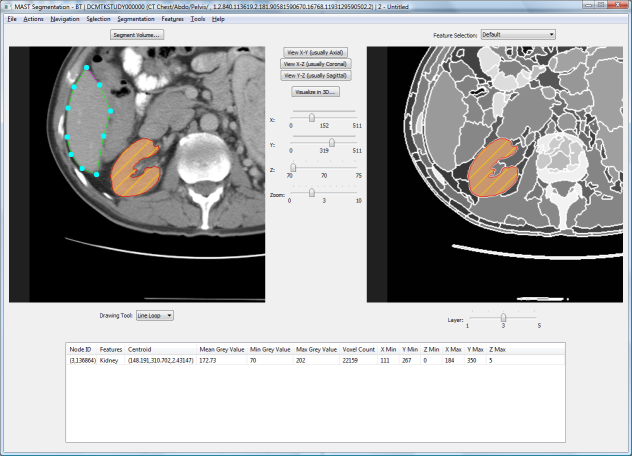
\includegraphics[height=.25\textheight]{introduction/introduction-millipede-seg-windows.png}}%
	%
	\\ \vspace{5mm}
	%
	\subfigure[\emph{millipede} running on Linux (Ubuntu)]
	{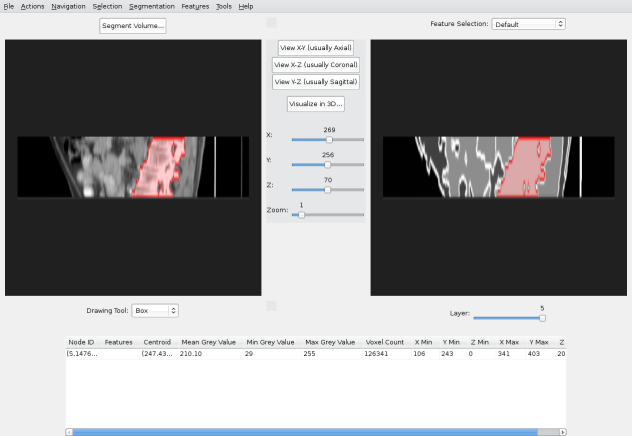
\includegraphics[height=.25\textheight]{introduction/introduction-millipede-seg-linux.png}}%
	%
	\\ \vspace{5mm}
	%
	\subfigure[\emph{millipede} running on Mac OS X (Snow Leopard)]
	{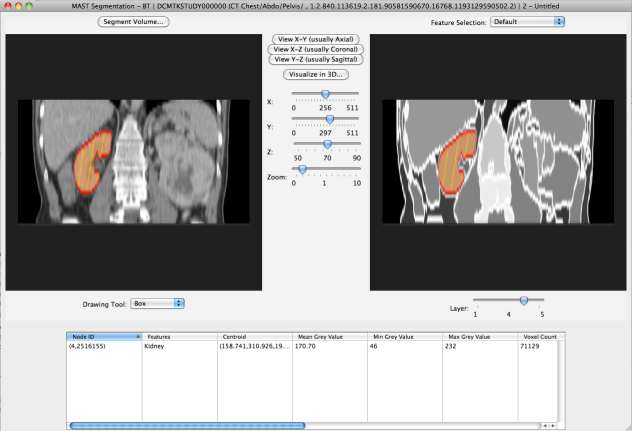
\includegraphics[height=.25\textheight]{introduction/introduction-millipede-seg-macosx.png}}%
\caption{The final segmentation system I developed, known as \emph{millipede}, is cross-platform.}
\label{fig:introduction-millipede-seg}
\end{stusubfig}
%---

The final system, \emph{millipede}, is built using a cross-platform build framework called CMake, and runs on Microsoft Windows, Linux and Mac OS X (see Figure~\ref{fig:introduction-millipede-seg}). It allows the user to segment slices from a CT (or MRI) series either as a 3D volume, or as individual axial, coronal or sagittal slices, in all cases producing a single image partition forest for the entire image volume used. Among many other improvements, it supports far better automatic feature identification, this time in 3D, and has built-in tools for validation. It can also visualize the feature identification results as a Phong-lit 3D mesh (see Figure~\ref{fig:introduction-millipede-vis}).

%---
\stufigex{height=6cm}{introduction/introduction-millipede-vis.png}{Visualizing the results of the automatic feature identification techniques in \emph{millipede} as a Phong-lit 3D mesh. Six features are visible: the aorta (red), right kidney (yellow), liver (purple), ribs (pale green), spine (pale blue) and spinal cord (slightly darker blue).}{fig:introduction-millipede-vis}{t}
%---

The original contributions made by this dissertation, then, are as follows:

\begin{enumerate}
\item A hierarchy of undoable operations to mutate partition forests, and their integration into a graphical user interface (\S\ref{sec:ipfs-mutatingalgorithms}).
\item A subtree-based, self-updating partition forest selection data structure (\S\ref{sec:ipfs-selections}).
\item A simple, edge-preserving image filter -- known as a \emph{spatially-variant Gaussian filter} (\S\ref{subpara:svgf}).
\item A new, implementation-invariant algorithm for the waterfall transform on minimum spanning trees (\S\ref{?}).
\item A technique to construct image partition forests for 3D images, making use of the existing watershed and waterfall transforms (\S\ref{?}).
\item Novel feature identification techniques for 2D and 3D abdominal CT scans (Chapter~\ref{chap:featureid}).
\item The implementation of the \emph{centipede} and \emph{millipede} segmentation, feature identification and 3D visualization systems in C++.
\end{enumerate}

\iffalse

\begin{itemize}

\item Attempts have been made to solve segmentation and feature identification in abdominal CT scans before, e.g.~...
\item But the limitations of these various methods are ...?
\item In other imaging subfields (including some of medical imaging) partition trees have been applied to good effect to represent images -- including some trees based on watershed (but not waterfall)
\item In some cases, attempts have been made to allow selection of regions in such a tree via cuts, etc.
\item What has not been done before is to build an explicit partition hierarchy using both the watershed and waterfall transforms and to use it (in combination with novel algorithms) to facilitate editing of segmentation results by the user
\item Furthermore, no-one has tried multi-layer region growing techniques for feature identification before (for that matter, I'm not sure they've tried multi-layer feature identification techniques period)
\item These, then, provide my `niche' (occupying it)
\item It is an interesting approach to try because it in principle combines the automation of morphological techniques with the previously untapped editing potential of partition hierarchies
\item Over the course of this dissertation, I will argue that it is also a useful approach, based on my results
\item Specifically, I aim to defend the thesis statement that...

\end{itemize}

\fi

%---
\section*{Dissertation Organisation}

TODO: This section needs a rewrite

The remainder of this dissertation is organised as follows.

\textbf{Chapter~\ref{chap:background}} surveys the fields of segmentation and feature identification, and discusses some of the varied uses of partition hierarchies throughout computer science, with the intention of both placing my own techniques in context and providing the foundations for later discussion.

\textbf{Chapter~\ref{chap:methodology}} describes my research methodology in more detail, focusing in particular on the question of the appropriateness of my goals and the methods I chose to achieve them.

\textbf{Chapter~\ref{chap:ipfs}} describes partition forests, the key data structure I used to represent segmented images, and introduces novel algorithms I have developed for editing them and selecting nodes in multiple layers within them.

\textbf{Chapter~\ref{chap:segmentation}} shows how partition forests can be constructed from images using existing segmentation approaches such as the watershed and waterfall transforms. It looks at three different ways in which the waterfall transform can be implemented: an algorithm due to Marcotegui and Beucher \cite{marcotegui05}, a new tree-based algorithm due to my colleague Chris Nicholls \cite{nicholls09}, and my own novel tree-based approach, presented here for the first time, that handles minimal plateaux in a robust manner.

\textbf{Chapter~\ref{chap:featureid}} shows how feature identification algorithms, including a novel multi-layer region growing method, can be applied to the partition forest in order to automatically segment certain abdominal features. It also illustrates how the results of the segmentation and feature identification processes can be useful in solving real-world problems such as visualizing abdominal organs in three dimensions and calculating organ volumes.

\textbf{Chapter~\ref{chap:assessment}} assesses and validates the contributions made elsewhere in the dissertation (see below) and summarises my case supporting the thesis statement.

\textbf{Chapter~\ref{chap:conclusions}} discusses potential avenues for further work, and concludes the dissertation.

\textbf{Appendix~\ref{chap:appendixds}} provides information on basic structures such as disjoint set forests and minimum spanning trees.